\documentclass[11pt]{article}

\usepackage{graphicx}

\usepackage[margin={.1in,.1in}]{geometry}
 
\begin{document}


 



\begin{subsection}{Types of Transfer functions:}

$\tilde{H(\omega)} =  Voltage \; gain = \frac{\tilde{V_o}}{\tilde{V_i}}$ \
$\tilde{H(\omega)} =  Current  \; gain = \frac{\tilde{I_o}}{\tilde{I_i}}$ \
$\tilde{H(\omega)} =  Transfer \; Impedance = \frac{\tilde{V_o}}{\tilde{I_i}}$ \

$\tilde{H(\omega)} =  Transfer \; admittance = \frac{\tilde{I_o}}{\tilde{V_i}}$ \


\begin{subsection}{General form of Transfer Function:}

$\tilde{H(\omega)} = \frac{\tilde{N(\omega)}}{\tilde{D(\omega)}}$

Where $\tilde{D(\omega_{poles})} = 0 $ //
	$\tilde{N(\omega_{zeros})} = 0$ 
			

\end{subsection}
\end{subsection}


\begin{subsection}{Definition of the bel:}

G = Number of bels = $log_{10}(\frac{P_o}{P_i})$

$G_{dB} =  10 \cdot log_{10}(\frac{P_o}{P_i})$

$G_{dB} = 20 \cdot log_{10}(\frac{I_o}{I_i}) $

$G_{dB} = 20 \cdot log_{10}(\frac{V_o}{V_i}) $


\end{subsection}




\begin{section}{RLC Series resonant circuit}


$\tilde{Z} = \tilde{H(s)} = R + j \omega L + \frac{1}{j \omega C} $

 when $(\;  Im(\tilde{Z}(\omega_o)) = 0 \;\;)$ \ \   

 $\omega_o = \frac{1}{\sqrt{LC}}$
    
    
\begin{subsection}{ Characteristics } 

$\omega_1 = - \frac{R}{2L} + \sqrt{({\frac{R}{2L}})^2 + \frac{1}{LC}}$ \

$\omega_2 = \frac{R}{2L} + \sqrt{({\frac{R}{2L}})^2 + \frac{1}{LC}}$ \

$\omega_o = \sqrt{\omega_1 \cdot \omega_2}$ \ 

$B = \omega_2 - \omega_1$ \ 

$Q = 2 \pi \frac{ maxium energy stored}{total energy lost per cycle at resonance} = 2\pi \frac{E_s}{E_D}$ \

\

$E_s = \frac{1}{2}L i^2 + \frac{1}{2}C v_c^2$ \

Assuming that: $v_c(t) =  V_C sin(\omega t)$ \

$i = C \frac{dv_c}{dt} = \omega C V_c sin^2(\omega t)$ \

$E_s(\omega_o) = \frac{1}{2}C V_c^2$ \

 $ E_D(\omega_o) = (i(\omega_o)^2 * R) (\frac{1}{f_o}) $ \

 $Q = \frac{\omega_o L}{R} = \frac{1}{\omega_o RC}$ \

 $B = \frac{L}{R} = \frac{\omega_o}{Q}$ \

\end{subsection}
\end{section}



\begin{section}{RLC Parallel resonant circuit}

$\tilde{Z} = \tilde{H(s)} = R + j \omega L + \frac{1}{j \omega C} $

 when $(\;  Im(\tilde{Z}(\omega_o)) = 0 \;\;)$ \ \ 

    $\omega_o = \frac{1}{\sqrt{LC}}$ \
    

\begin{subsection}{Characteristics } \

$\omega_1 = - \frac{1}{2RC} + \sqrt{({\frac{1}{2RC}})^2 + \frac{1}{LC}}$ \

$\omega_2 = \frac{1}{2RC} + \sqrt{({\frac{1}{2RC}})^2 + \frac{1}{LC}}$

$Q = \frac{omega_o}{B} = \omega_o RC = \frac{R}{\omega_o L}$

$B = \frac{1}{RC} $



\end{subsection}
\end{section}

\begin{subsection}{For SERIES AND PARALLEL:}

$\omega_1 = \omega_o [ \sqrt{({\frac{1}{2Q}})^2 - \frac{1}{2Q}}] $ \


$\omega_2 = \omega_o [ \sqrt{({\frac{1}{2Q}})^2 + \frac{1}{2Q}}] $ \

\end{subsection}



\begin{section}{Passive Filters}




\begin{figure}
	    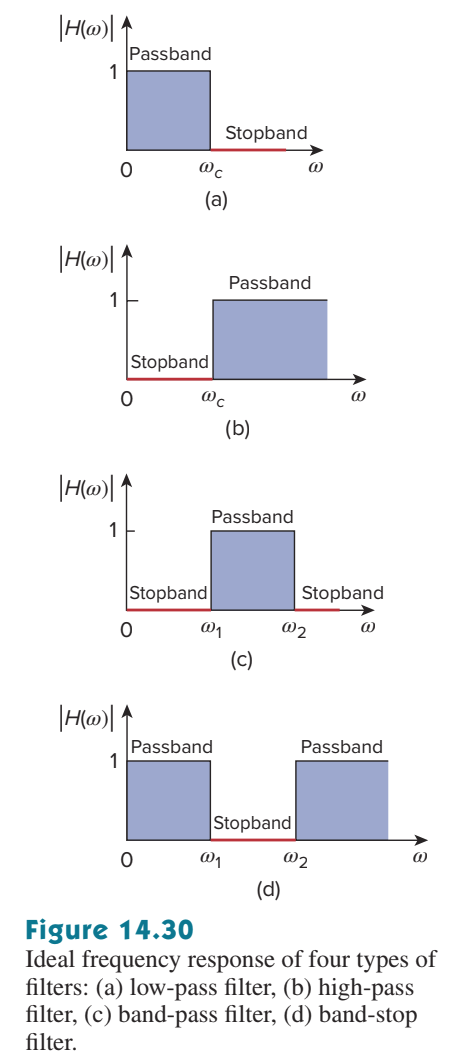
\includegraphics[width=.4\textwidth]{passiveFilterGraph.png}
    \end{figure}


\begin{subsection}{Low Pass Filter}
RC:
\begin{figure}
 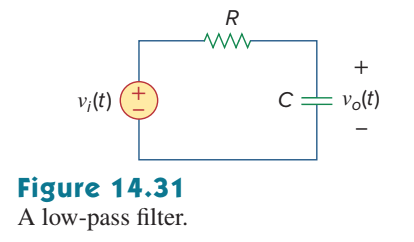
\includegraphics[bb=0 0 30 30]{LPF_RC.png}
\end{figure}

$\tilde{H(\omega)} = \frac{\tilde{V_o}}{\tilde{V_i}} = \frac{1}{1+ j \omega * R * C} $

$\omega_c = \frac{1}{RC}$

\end{subsection}

\begin{subsection}{High Pass Filter}
RC:

\begin{figure}
	 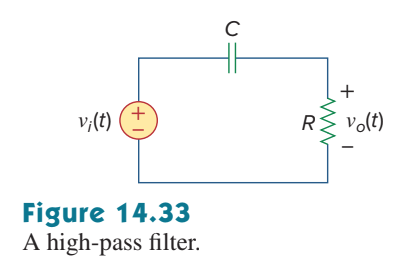
\includegraphics[bb=0 0 30 30]{HPF_RC.png}
 \end{figure}

 $\tilde{H(\omega)} = \frac{\tilde{V_o}}{\tilde{V_i}} = \frac{j \omega R C}{1+ j \omega * R * C} $

 $\omega_c = \frac{1}{RC}$

\end{subsection}

\begin{subsection}{Band Pass Filter}

\begin{figure}
	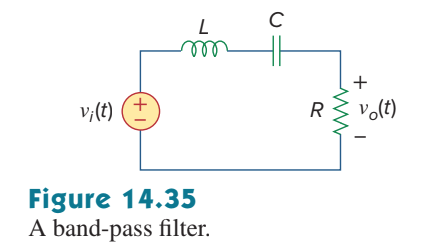
\includegraphics[bb=0 0 30 30]{BPF_RLC.png}
\end{figure}

$\tilde{H(\omega)} = \frac{\tilde{V_o}}{\tilde{V_i}} = \frac{ R }{R+ j (\omega L - \frac{1}{\omega C})} $

$\omega_o = \frac{1}{\sqrt{LC}}$

\end{subsection}

\begin{subsection}{Band Stop Filter}

\begin{figure}
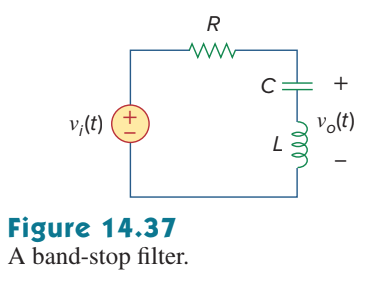
\includegraphics[bb=0 0 30 30]{BSF_RLC.png}
\end{figure}

$\tilde{H(\omega)} = \frac{\tilde{V_o}}{\tilde{V_i}} = \frac{ j(\omega L - \frac{1}{\omega C}) }{R+ j (\omega L - \frac{1}{\omega C})} $

$\omega_o = \frac{1}{\sqrt{LC}}$

\end{subsection}



\end{section}
 

\end{document}

